% =============================================================================
% Solar Filament Segmentation Challenge 2026 -- technical report
% 主催者の Overleaf テンプレート（https://www.overleaf.com/read/vjztpvrnbrdh）をそのまま使用。
% テンプレートの固定文（Introduction の最初の 2 文、節の名前、Acknowledgment、subtitle）は変更しない。
% 本文は Acknowledgment と References を除いて 4 ページ以内。
% 図は OOF 出力から report_figs3.py（pipeline, gallery, evald）と report_figs4.py（agree = concept, evid = agree）で生成（707 枚、最終版の設定）。
% 専門家の一致の数値は report_agree.py / report_agree2.py、選別の寄与は report_sel.py。
% 数値は全て最終提出の構成（しきい値 0.45、特徴 32 個、規則 0.18 / 0.6）で、scorer は fold ごとに学習した値。
% =============================================================================

\documentclass[sigconf]{acmart}
% =============================================================================
% Template setup — participants normally do not edit this file.
% Author content belongs in main.tex; citations belong in main.bib.
% \documentclass lives in main.tex so Overleaf does not treat this file as root.
% =============================================================================

% --- Competition / non-ACM-submission friendly rights metadata -------------
\setcopyright{none}
\settopmatter{printacmref=false}
\acmConference[Kaggle Competition]{Filament Segmentation Challenge}{2026}{\href{https://www.kaggle.com/competitions/filament-segmentation-2026}{kaggle.com/competitions/filament-segmentation-2026}}
\acmBooktitle{Competition Report}
\acmDOI{}
\acmISBN{}

% --- Author guidance text --------------------------------------------------
% \guide{...} is gray italic while \guideStyletrue; omitted from the PDF if false.
% Flip the switch in main.tex after % =============================================================================
% Template setup — participants normally do not edit this file.
% Author content belongs in main.tex; citations belong in main.bib.
% \documentclass lives in main.tex so Overleaf does not treat this file as root.
% =============================================================================

% --- Competition / non-ACM-submission friendly rights metadata -------------
\setcopyright{none}
\settopmatter{printacmref=false}
\acmConference[Kaggle Competition]{Filament Segmentation Challenge}{2026}{\href{https://www.kaggle.com/competitions/filament-segmentation-2026}{kaggle.com/competitions/filament-segmentation-2026}}
\acmBooktitle{Competition Report}
\acmDOI{}
\acmISBN{}

% --- Author guidance text --------------------------------------------------
% \guide{...} is gray italic while \guideStyletrue; omitted from the PDF if false.
% Flip the switch in main.tex after % =============================================================================
% Template setup — participants normally do not edit this file.
% Author content belongs in main.tex; citations belong in main.bib.
% \documentclass lives in main.tex so Overleaf does not treat this file as root.
% =============================================================================

% --- Competition / non-ACM-submission friendly rights metadata -------------
\setcopyright{none}
\settopmatter{printacmref=false}
\acmConference[Kaggle Competition]{Filament Segmentation Challenge}{2026}{\href{https://www.kaggle.com/competitions/filament-segmentation-2026}{kaggle.com/competitions/filament-segmentation-2026}}
\acmBooktitle{Competition Report}
\acmDOI{}
\acmISBN{}

% --- Author guidance text --------------------------------------------------
% \guide{...} is gray italic while \guideStyletrue; omitted from the PDF if false.
% Flip the switch in main.tex after \input{preamble}.
%
% Do not use \guide{...} for \email{...}.
\usepackage{xcolor}
\newif\ifguideStyle
\guideStyletrue
\newcommand{\guide}[1]{%
  \ifguideStyle
    {\color{gray!65}\itshape #1}%
  \fi
}

% --- Math ------------------------------------------------------------------
% Do NOT load amssymb (or amsfonts): acmart already loads newtxmath, which
% defines the same symbols (e.g. \Bbbk) and causes a conflict on Overleaf.
% amsmath is already provided by acmart; mathtools extends it.
\usepackage{mathtools}

% --- Figures ---------------------------------------------------------------
% graphicx is already loaded by acmart
\usepackage{subcaption}

% --- Tables ----------------------------------------------------------------
% booktabs is already loaded by acmart
\usepackage{tabularx}
\usepackage{multirow}

% --- Bibliography style is set in main.tex (ACM-Reference-Format) ----------
.
%
% Do not use \guide{...} for \email{...}.
\usepackage{xcolor}
\newif\ifguideStyle
\guideStyletrue
\newcommand{\guide}[1]{%
  \ifguideStyle
    {\color{gray!65}\itshape #1}%
  \fi
}

% --- Math ------------------------------------------------------------------
% Do NOT load amssymb (or amsfonts): acmart already loads newtxmath, which
% defines the same symbols (e.g. \Bbbk) and causes a conflict on Overleaf.
% amsmath is already provided by acmart; mathtools extends it.
\usepackage{mathtools}

% --- Figures ---------------------------------------------------------------
% graphicx is already loaded by acmart
\usepackage{subcaption}

% --- Tables ----------------------------------------------------------------
% booktabs is already loaded by acmart
\usepackage{tabularx}
\usepackage{multirow}

% --- Bibliography style is set in main.tex (ACM-Reference-Format) ----------
.
%
% Do not use \guide{...} for \email{...}.
\usepackage{xcolor}
\newif\ifguideStyle
\guideStyletrue
\newcommand{\guide}[1]{%
  \ifguideStyle
    {\color{gray!65}\itshape #1}%
  \fi
}

% --- Math ------------------------------------------------------------------
% Do NOT load amssymb (or amsfonts): acmart already loads newtxmath, which
% defines the same symbols (e.g. \Bbbk) and causes a conflict on Overleaf.
% amsmath is already provided by acmart; mathtools extends it.
\usepackage{mathtools}

% --- Figures ---------------------------------------------------------------
% graphicx is already loaded by acmart
\usepackage{subcaption}

% --- Tables ----------------------------------------------------------------
% booktabs is already loaded by acmart
\usepackage{tabularx}
\usepackage{multirow}

% --- Bibliography style is set in main.tex (ACM-Reference-Format) ----------


% Guide styling: \guideStyletrue = show gray italic hints; \guideStylefalse = omit them
\guideStylefalse

\renewcommand{\dbltopfraction}{0.9}
\renewcommand{\dblfloatpagefraction}{0.9}
\begin{document}

\title{What Experts Agree On: Solar Filament Segmentation Under Annotator Disagreement}  % Replace this with your title
\subtitle{A Solution to the Solar Filament Segmentation Challenge 2026} % DO NOT CHANGE


\author{Firstname Lastname}   % <- 著者1
\affiliation{%
  \institution{Your Institution}
  \city{City}
  \country{Japan}
}
\email{first.author@example.com}   % <- Replace with your own email

\author{Second Author}   % <- 著者2
\affiliation{%
  \institution{Your Institution}
  \city{City}
  \country{Japan}
}
\email{second.author@example.com}  % <- Replace with your own email

\begin{abstract}
    Experts do not agree on what a solar filament is.
    On the 296 training images of the Solar Filament Segmentation Challenge~2026 that were annotated by more than one expert, one expert scored against another reaches a Panoptic Quality (PQ) of 0.340, and 37\,\% of an expert's filaments are matched (IoU~$>0.5$) by no other expert.
    A model therefore cannot score by imitating one expert; what it can learn is what experts agree on.
    Our pipeline is trained on every expert's annotation at each stage: a full-resolution detector proposes candidates, a second stage re-draws each candidate from every expert's outline of it, and a scorer estimates the share of experts who would accept the result.
    Out of fold it reaches PQ~0.458 (public leaderboard 0.40).
    It hits 89\,\% of the filaments that all other experts drew and 35\,\% of those that none did; on filaments confirmed by a second expert it hits 84\,\% where a third expert hits 73\,\%; 70\,\% of its misses are filaments that no other expert matched, and 57\,\% of its false positives against one expert match a filament of another expert of the same image.
    Only the competition training data was used.
\end{abstract}

\begin{teaserfigure}
    \centering
    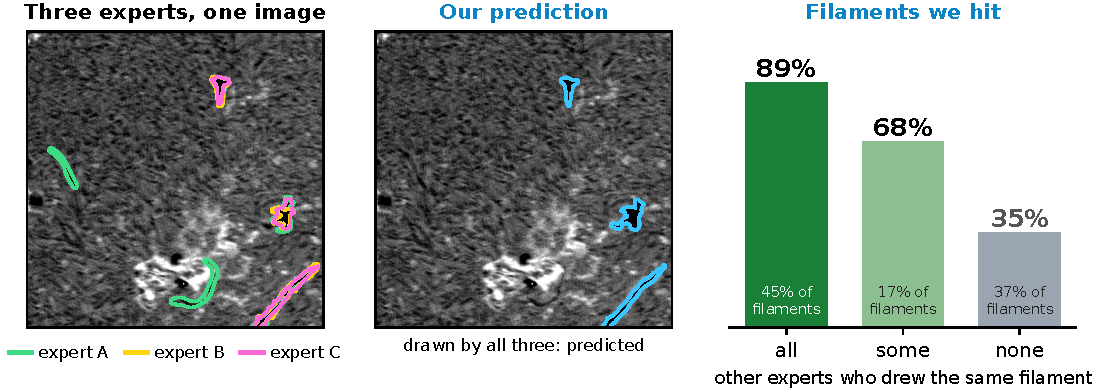
\includegraphics[width=\textwidth]{figures/concept}
    \caption{Experts do not agree on what a filament is; the model predicts what they agree on. Left: the outlines of the three experts who annotated this image, one colour per expert. Three filaments were drawn by all of them and two by one expert only. Centre: our out-of-fold prediction for the same region. Right: share of the experts' filaments that our prediction hits (IoU~$>0.5$), by how many of the other experts of the image drew the same filament (IoU~$>0.5$ between experts); 296 images with two or three experts, 4{,}993 filaments. The example was chosen by hand.}
    \label{fig:concept}
\end{teaserfigure}

\maketitle

% ==================================== %
%              INTRODUCTION            %
% ==================================== %
\section{Introduction}
    This report goes over the details of our submitted solution to the Solar Filament Segmentation Challenge~2026 \cite{filament-segmentation-2026}. The challenge, launched on July~10,~2026, is organized by the Earth-Space AI Research (ESAIR) Lab\footnote{\href{https://www.esairlab.com/home}{www.esairlab.com/}}. This challenge utilizes the MAGFiLO dataset for evaluation of the segmentation algorithms \cite{ahmadzadeh2024dataset}.
    % --- ここから自分の文 ---

    The metric, Panoptic Quality \cite{kirillov2019panoptic}, compares a prediction with one expert at a time and counts a filament only if the two outlines overlap by IoU~$>0.5$.
    In MAGFiLO, 296 of the 707 training images were annotated by two or three experts, which allows a question that is usually left open: how well does an expert do on this metric?
    Scored against each other, experts reach PQ~0.340.
    Of their 4{,}993 filaments on these images, 45\,\% are matched by all other experts of the image, 17\,\% by some, and 37\,\% by none. Among the last group, 64\,\% are partly overlapped by another expert's filament (the same structure, outlined or divided differently) and 36\,\% were drawn by nobody else (Fig.~\ref{fig:concept}, left).

    This has two consequences, and they organise the report.
    \emph{For the method:} a submitted instance earns, in expectation over experts, the share of experts who match it times the IoU of the match. The best prediction is therefore not one expert's annotation but the filaments, and the outlines, that experts have in common. We train every stage on all experts' annotations: the detector on each expert's mask of an image, the second stage on each expert's outline of the same candidate, and the scorer directly on the share of experts who match (Sec.~\ref{sec:methodology}).
    \emph{For the evaluation:} an error against one expert is not always an error. We therefore read every result against expert agreement (Sec.~\ref{sec:agreement}; Fig.~\ref{fig:concept}, right).

    The components themselves are standard: a segmentation network, per-instance refinement of a coarse mask \cite{cai2018cascade,kirillov2020pointrend} and mask scoring \cite{huang2019msrcnn}. What we contribute is the measurement of how expert agreement limits and structures the score on this dataset, a pipeline whose training targets follow from it, and an account of which of the remaining errors are the model's and which lie within the range in which experts differ.

    \textbf{Use of public material.}
    The Focal+Dice loss of the detector was suggested in the competition forum \cite{filament-segmentation-2026}.
    Four elements follow the public notebook of Kaggle user \emph{tushhaaarrrr} \cite{tushhaaarrrr2026filseg}: pairing UNet++ ResNet-34 with a ConvNeXt-T U-Net as refiners, keeping all refined components that touch the candidate, the hurdle form of the instance score, and weighting scorer rows by the number of experts.
    We re-implemented them and kept each only after it improved our out-of-fold PQ (about $+0.009$ together).
    We used no external images, magnetograms or temporally adjacent observations.


% ==================================== %
%              METHODOLOGY             %
% ==================================== %
\section{Methodology}\label{sec:methodology}

    \begin{figure*}[t]
        \centering
        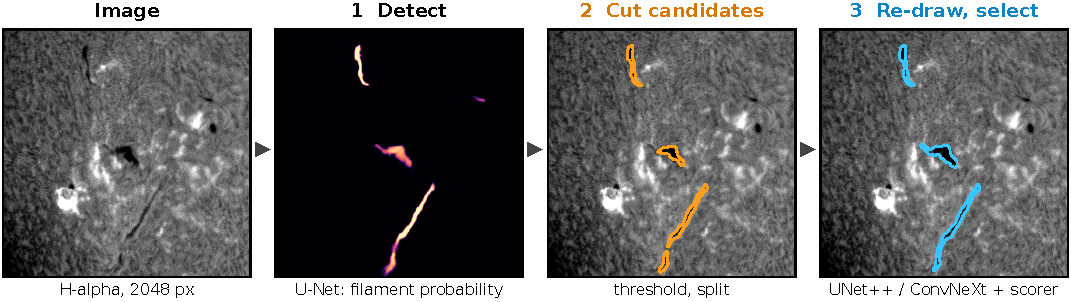
\includegraphics[width=\textwidth]{figures/pipeline}
        \caption{The pipeline on a 640\,px crop of a training image (out-of-fold). From left: input; Stage~1 probability map; candidates (orange) cut from the map; final instances (blue) after re-drawing, scoring and 0.5\,px erosion. The small candidate at the bottom is not kept. Settings are given in Sec.~\ref{sec:methodology}.}
        \label{fig:pipeline}
    \end{figure*}

    \subsection{Data, validation and pre-processing}
        The training set has 707 full-disk GONG H-$\alpha$ images (2048$\times$2048) with 1{,}154 image--expert annotation sets (8{,}199 filaments); 411 images have one expert, 145 two and 151 three. The test set has 180 images.
        Every image--expert pair is one training sample, so an image with three experts appears three times with three targets, as in the scoring.
        Images are split (by image) into 5 folds with a fixed seed, and every model is trained 5 times. All numbers in this report are \emph{out-of-fold} (OOF): each training image is predicted by models that never saw it, and scored against every expert with the organizers' evaluation code.
        Images are used at native resolution as one channel, without flat-fielding or limb-darkening correction.
        Augmentation is the dihedral group (flips, $90^\circ$ rotations) and an affine intensity change ($\times[0.85,1.15]$, $\pm15$ grey levels).

    \subsection{Stage 1: candidates}\label{sec:stage1}
        The detector is a U-Net \cite{ronneberger2015unet} with an ImageNet-pretrained ResNet-34 encoder \cite{he2016resnet} from Segmentation Models PyTorch \cite{iakubovskii2019smp}, trained on 1024\,px crops of the 2048\,px image (batch~4, 40 epochs, AdamW, weight decay $10^{-4}$, one-cycle schedule peaking at $3\cdot10^{-4}$, mixed precision). 70\,\% of the crops are centred on a random annotated filament and 30\,\% are uniform over the disk.
        The loss is Focal \cite{lin2017focal} ($\gamma=2$, weight~10) plus soft Dice.
        The same image is shown with each expert's mask, so the detector is trained towards all experts at once.
        Inference averages the 5 folds and 8 dihedral views in probability space.

        Candidates are cut from the averaged map $p$ by hysteresis: connected components of $p\ge0.15$ that contain a pixel with $p\ge0.8$; the mask of each is $p\ge0.6$, closed with radius~2.
        Fragments whose end-points are within 30\,px and whose end directions agree within $30^\circ$ (last 20\,px of the skeleton, elongation $\ge3$) are joined, because PQ counts a split filament as two errors. Components below 25\,px$^2$ or outside 0.9 of the disk radius are removed.

    \subsection{Stage 2: re-drawing each candidate}\label{sec:stage2}
        A threshold on the pixel map follows the dark core and gives masks smaller than the experts' outlines (median area ratio 0.93, Sec.~\ref{sec:stages}). The second stage draws each candidate again as an expert would.
        Each candidate is cropped with a square window of side $1.3\,s+48$\,px ($s$: its extent) and resized to 256$\times$256, so that every filament, short or long, fills the same part of the input.
        The network receives four channels: the image, the Stage-1 probability map, the candidate, and the union of all other candidates. The last two tell it \emph{which} filament to draw and which neighbours to leave alone.
        The target is one expert's filament: for every expert of the image, the ground-truth filament that best overlaps the candidate (IoU~$\ge0.2$). One (candidate, expert) pair is one sample, so the network sees the same crop with up to three outlines and cannot fit the habit of one expert.
        Candidates and probability maps used for training are OOF, so the refiner never sees a Stage-1 output that was fitted to its own target.

        Two refiners are trained per fold, UNet++ \cite{zhou2018unetpp} with ResNet-34 and a U-Net with a ConvNeXt-T encoder \cite{liu2022convnext} (Focal+Dice, 25 epochs, batch~32, dihedral augmentation, 10--20 min per fold).
        At inference their outputs are averaged over the two architectures, the 5 folds and 4 rotations, thresholded at 0.45 and pasted back at full resolution. Connected components that touch the candidate are kept; where two re-drawn filaments overlap, the pixel goes to the higher probability; a candidate whose re-drawn area falls below 30\,\% of its own is kept as it was.

    \subsection{Scoring and selection}\label{sec:scorer}
        Averaged over the experts of an image, a submitted instance earns $h\cdot m$ in the numerator of PQ and costs half an error otherwise, with $h$ the share of experts with a matching filament and $m$ the mean IoU of the matches.
        Two histogram gradient-boosting models estimate $h$ and $m$ from OOF candidates, each row weighted by the number of experts of its image; the selection target is thus expert agreement itself.
        They use 20 per-instance features (size and shape; probability statistics inside and in a ring around the instance, including the spread between the five folds; contrast against the surroundings; distance from disk centre and from the nearest candidate) and 12 \emph{consistency} features taken from the re-drawing: statistics of the refiner probability inside the mask, the fraction of undecided pixels, the IoU and area ratio between candidate and re-drawn mask, and the differences between the two architectures and between rotations.
        These features report where the re-drawing networks, trained on several experts' outlines, do not settle.
        An instance is kept if $\hat h\hat m\ge0.18$ and its mean Stage-1 probability is $\ge0.6$. Kept masks are eroded by 0.5\,px, never overlap, and are written as COCO RLE.


% ==================================== %
%              EVALUATION              %
% ==================================== %
\section{Evaluation}\label{sec:evaluation}

    \subsection{Evaluation strategy}
        All numbers are OOF on the 707 training images against all 1{,}154 annotation sets. The scorer is cross-fitted on the same 5 folds, and rules are chosen on 4 folds and scored on the 5th.
        A change is accepted only if a paired bootstrap over images \cite{efron1979bootstrap} (5{,}000 resamples) puts the 95\,\% interval of the PQ difference above zero; single-fold differences of $\pm0.006$ occur from the random seed alone.
        For the agreement analysis we use the 296 images with two or three experts. Each expert is scored against each other expert of the same image (1{,}196 ordered pairs), and each expert filament is labelled by how many of the other experts have a filament with IoU~$>0.5$ to it: all, some, or none.

    \begin{figure*}[t]
        \centering
        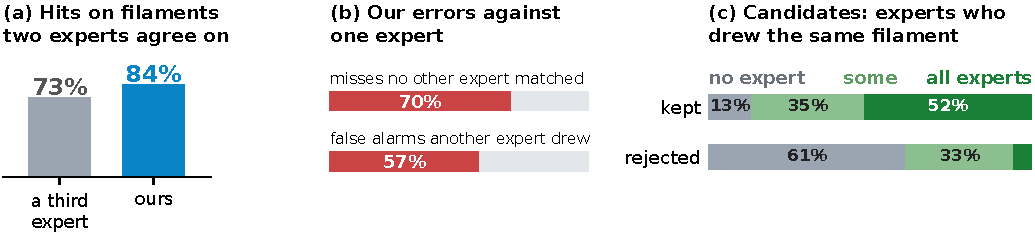
\includegraphics[width=\textwidth]{figures/agree}
        \caption{Reading the errors against expert agreement (multi-expert training images, out-of-fold). (a)~Filaments of one expert that a second expert confirmed: share hit by the third expert and by us. (b)~Our misses that no other expert matched, and our false positives that match another expert of the same image. (c)~Candidates kept and rejected by the scorer, by how many experts have a matching filament.}
        \label{fig:agree}
    \end{figure*}

    \begin{figure*}[t]
        \centering
        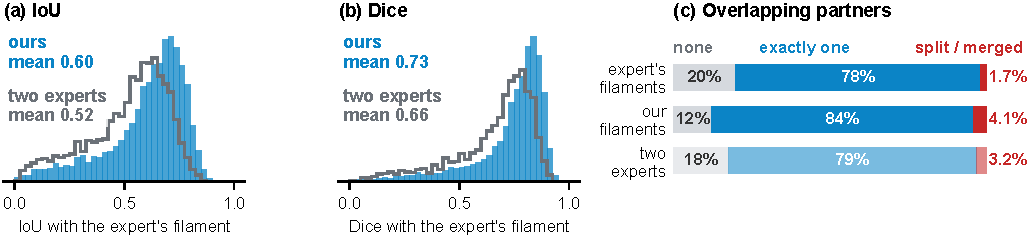
\includegraphics[width=\textwidth]{figures/eval_dist}
        \caption{The diagnostics of the organizers' self-evaluation notebook on the 707 training images, out-of-fold (blue), and for one expert scored against another (gray line in a, b; pale row in c). (a, b)~IoU and Dice of all overlapping (ground truth, prediction) pairs. (c)~Share of filaments with no, exactly one, or several overlapping partners (a split or a merge).}
        \label{fig:evaldist}
    \end{figure*}

    \begin{figure}[t]
        \centering
        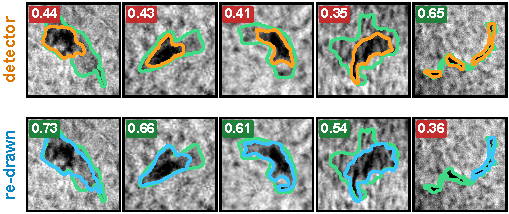
\includegraphics[width=\columnwidth]{figures/gallery}
        \caption{Stage-1 candidates (top, orange) and the same candidates re-drawn (bottom, blue) against one expert's outline (green). Badge: IoU with that expert, green if a hit ($>0.5$). Columns 1--4 are taken by hand from the largest gains, column 5 from the largest losses.}
        \label{fig:gallery}
    \end{figure}

    \subsection{Agreement: between experts, and with the model}\label{sec:agreement}
        On the 296 multi-expert images our prediction reaches PQ~0.456; one expert against another reaches 0.340 (SQ~0.634, RQ~0.536).
        The model is not better than an expert; it is closer to all of them than they are to each other, which is what the metric rewards.

        \emph{The model follows the consensus.}
        It hits 89\,\% of the filaments that all other experts drew (2{,}270 filaments), 68\,\% of those that some drew (868) and 35\,\% of those that no other expert matched (1{,}855); the mean IoU of the overlaps falls in the same order, 0.68, 0.59 and 0.49 (Fig.~\ref{fig:concept}).

        \emph{On confirmed filaments it agrees with an expert more often than a colleague does.}
        On the 151 images with three experts, take a filament of one expert that a second expert confirmed (3{,}172 cases). The third expert hits it in 73\,\% of the cases, our prediction in 84\,\% (Fig.~\ref{fig:agree}a); where both hit, the mean IoU is 0.645 for the third expert and 0.703 for ours.

        \emph{Most errors against one expert are disagreements between experts.}
        70\,\% of our misses are filaments that no other expert of the image matched, and 14\,\% are filaments that all others matched. Of our 1{,}425 false positives against one expert, 57\,\% match a filament of another expert of the same image (Fig.~\ref{fig:agree}b).
        What is clearly the model's own error is smaller: 11\,\% of the consensus filaments are missed, and 13\,\% of the submitted instances match no expert of the image (Fig.~\ref{fig:agree}c).

    \subsection{What each stage contributes}\label{sec:stages}
        \emph{Re-drawing} (Fig.~\ref{fig:gallery}).
        Among the 6{,}771 (candidate, expert) pairs with IoU~$\ge0.2$, 398 cross the matching threshold upwards when the candidate is re-drawn and 120 downwards. The candidate's area is on median 0.93 of the expert's, the re-drawn mask's 1.00: the thresholded map follows the dark core, and the experts also include the fainter periphery, barbs and thin ends.
        The share of expert filaments hit by some candidate rises in every agreement class: from 88.9 to 90.7\,\% (all), 68.0 to 72.4\,\% (some) and 36.5 to 40.9\,\% (none). The gain is largest where experts differ, that is, where the outline rather than the presence of the filament decides the match.

        \emph{Selection.}
        Submitting every re-drawn candidate gives PQ~0.446; a fixed rule on the mean Stage-1 probability and the distance from disk centre 0.454; the scorer 0.458.
        Of the candidates the scorer rejects on multi-expert images, 61\,\% match no expert and 6\,\% match all; of those it keeps, 13\,\% and 52\,\% (Fig.~\ref{fig:agree}c).
        The 12 consistency features add $+0.0018$ (95\,\% interval $[0.0000, +0.0036]$, higher in all 5 folds), and pasting at 0.45 instead of 0.5 adds $+0.0051$ (interval $[+0.0022,$ $+0.0080]$).

    \begin{table}[t]
        \caption{PQ on the 707 training images (OOF) and on the public leaderboard ($\sim$90 test images, two decimals shown).}
        \label{tab:progress}
        \small
        \begin{tabular}{@{}lcc@{}}
            \toprule
            Method & OOF PQ & Public \\
            \midrule
            One expert scored against another & 0.340 & -- \\
            \midrule
            Candidates only: 2048\,px detector + scorer & 0.447 & -- \\
            + re-drawing (threshold 0.5) & 0.450 & 0.39 \\
            + threshold 0.45, re-tuned rule & 0.457 & 0.40 \\
            + consistency features (final) & \textbf{0.458} & \textbf{0.40} \\
            \bottomrule
        \end{tabular}
        \par\smallskip\footnotesize ``Candidates only'' uses its own best rule and no erosion, which is its best case.
    \end{table}

    \subsection{Results}
        The final model reaches PQ~0.458 on the 707 training images (SQ~0.681, RQ~0.673; 5{,}215 true positives, 2{,}078 false positives, 2{,}984 false negatives) and 0.40 on the public leaderboard (Table~\ref{tab:progress}).
        On the organizers' diagnostics (Fig.~\ref{fig:evaldist}) the mean IoU of overlapping pairs is 0.60 and the mean Dice 0.73 (experts: 0.52 and 0.66).
        Splits and merges are rare: 1.7\,\% of ground-truth filaments overlap two or more predictions and 4.1\,\% of predictions two or more filaments (experts: 3.2\,\%).
        Across submissions the public score was $0.87\pm0.02$ times the OOF PQ, so we chose the final submission by OOF PQ.
        Inference takes 3.6\,s per image on an RTX~4090 (detector 1.5\,s, candidates and re-drawing 1.3\,s, scoring and output 0.7\,s; 11~min for the 180 test images). Re-running the public repository reproduces the submitted file: 1{,}132 of 1{,}132 filaments, 1{,}121 pixel-identical, the rest with IoU~$>0.9$.

    \subsection{Limits and next steps}\label{sec:limits}
        \emph{Selection is the largest gap we can measure.} Keeping exactly the candidates whose true $h\cdot m$ is at least 0.18 would give PQ~0.513 instead of 0.458; the scorer's estimate correlates with it at 0.56. Predicting which candidates experts accept is where we would work next.
        \emph{Re-drawing has saturated in this design.} A third and fourth refiner architecture, 8-fold instead of 4-fold rotation averaging, wider or tighter crops and a per-candidate threshold each changed PQ by less than 0.001.
        When re-drawing fails, it over-reaches along a faint lane or into a neighbouring fragment (Fig.~\ref{fig:gallery}, right).
        \emph{Not everything is found.} 1{,}047 of the 8{,}199 expert filaments have no candidate at all, and the second stage cannot recover them.
        \emph{The agreement analysis has its own limit.} It rests on the 296 images with two or three experts; on an image with two experts, ``no other expert'' means one person, so the agreement classes are noisier there than on images with three.


% ==================================== %
%            ACKNOWLEDGMENT            %
% ==================================== %
\section{Acknowledgment}\label{sec:acknowledgment}
    % Do not change
    The organization of the Filament Segmentation Challenge 2026 is partially supported by the U.S. National Science Foundation (NSF) under Grant No. 2209912 and 2433781, directorate for Computer and Information Science and Engineering (CSE), and Office of Advanced Cyberinfrastructure (OAC), and Grant No. 2511630, AST Division Of Astronomical Sciences and MPS Directorate for Mathematical and Physical Sciences.

    The Filament Segmentation Challenge 2026 is sponsored by the U.S. National Science Foundation (NSF) National Solar Observatory (NSO).

    This work utilizes GONG data obtained by the NSO Integrated Synoptic Program, managed by the National Solar Observatory, which is operated by the Association of Universities for Research in Astronomy (AURA), Inc. under a cooperative agreement with the National Science Foundation and with contribution from the National Oceanic and Atmospheric Administration. The GONG network of instruments is hosted by the Big Bear Solar Observatory, High Altitude Observatory, Learmonth Solar Observatory, Udaipur Solar Observatory, Instituto de Astrofísica de Canarias, and Cerro Tololo Interamerican Observatory.

\bibliographystyle{ACM-Reference-Format}
\bibliography{main}

\end{document}
